\section{技术拆解与黏滞度量表}

量表要把一句“这项技术卡住了”，拆成可以逐格检查的判断：任务是什么，哪一段需要什么资源，反馈要等多久，改动会牵连谁，依据来自哪里。量表先提供约束画像；经过标定的数量模型再估计总体代价。

\subsection{拆解：找到可以独立检查的单元}

一个单元应当有可检查的输出，内部过程也应当具有相对一致的时间尺度。若同一单元同时容纳毫秒级计算与多年随访，平均值会遮住真正的约束。可以先用时间尺度的跨度辅助拆分：
\begin{equation}
\frac{\max_j\tau_j}{\min_j\tau_j}\leq\Lambda .
\label{eq:scale-lambda}
\end{equation}
$\tau_j$为子过程的特征时间，$\Lambda$为公开选定的拆解阈值。取$\Lambda$约为10，可以作为起点；是否继续拆分，还要看能否辨认新的机制，不能由一个数量级的界限直接决定。

单元分为两类。链上单元直接产生下一段使用的结果，例如制造电芯、完成试验、交付软件。界面单元连接外部系统，例如适航审定、采购接入、空域协调和服务接受。两类单元都可能因技术、组织与制度改进而变快，具体哪些部分能够提速，需要逐项查明。

\subsection{定级：先使用序数，再建立数量刻度}

表\ref{tab:scale-anchors}给出零到五级的示意锚点。级别表示同一坐标内约束由低到高，采用前应为具体任务确定判据，并附上证据。

\begin{table}[ht]
\centering
\caption{三个坐标的序数锚点}
\label{tab:scale-anchors}
{\small
\begin{tabularx}{\textwidth}{@{}lXXX@{}}
\toprule
等级 & 资源势垒$R$ & 时间刚性$T$ & 拓扑耦合$G$\\
\midrule
0 & 现有能力内的较小边际投入 & 相对任务可视为即时 & 局部改动，依赖很少\\
1 & 通用设备与常规供应可支持 & 短于主要运营周期 & 接口已知且较标准化\\
2 & 需要专用设备或材料 & 占用明显的运营时间 & 若干接口需要适配\\
3 & 需要显著资本、供应或基础设施投入 & 跨越重要计划或建设周期 & 多团队或供应商需要协调\\
4 & 关键投入稀缺，或须重大扩容 & 较长观察、更新或制度过程 & 多组织、标准或辖区相互影响\\
5 & 在所定边界内面临严重约束 & 远长于当前决策窗口 & 依赖广泛且难以隔离\\
\bottomrule
\end{tabularx}}
\end{table}

零级仍然消耗能量与材料，五级也不直接表示不可能。守恒律可以约束一项任务，却不能单独证明所有可选设计都已达到极限。表中的类别没有等距保证：时间差一级不自动等于十倍，资源差两级也不能直接换算成费用倍数。

若确有适当数据，可以另建连续刻度。例如明确规定
\begin{equation}
T=\log_{10}(\tau/\tau_0),
\qquad
\tau_{k+1}/\tau_k=10
\label{eq:scale-decade}
\end{equation}
时，级差才与时间数量级对应。这里的$\tau_0$是给定参照，不由序数表自动产生。资源也要选择同口径的实测量另行标定。

不确定性用相邻档位、置信区间或缺失证据报告。若仅能判断第$k$档与第$k+1$档之间尚不明确，就记录
\begin{equation}
R_i\in\{k,k+1\},
\label{eq:scale-fuzzy}
\end{equation}
并说明什么证据可以消除分歧。小数不能替代这份证据。

对有明确定义的依赖闭包规模$d_i$，可以采用一种计数分档：
\begin{equation}
G_i=\min\!\left\{5,\left\lfloor\log_{10}(1+d_i)\right\rfloor\right\}.
\label{eq:scale-G-def}
\end{equation}
图上可达、因果上受影响、必须同步修改、需要行政协调，是四种不同关系。闭包采用哪一种，必须先写清。计数也不能替代连接强度、关键节点与故障传播方式。

\subsection{合成：先合成实际量，再判断等级}

资源量在单位与边界一致时可以相加：
\begin{equation}
P_{\text{总}}=\sum_i P_i .
\label{eq:scale-R-agg}
\end{equation}
电力、材料、工时与资金各有账本；跨单位合成，需要公开的折算。对资源等级取加权平均，只会得到一个按所选规则形成的描述指数，不能据此恢复总资源需求。

时间必须按任务结构计算。严格串行的历时相加；同时开始且都须完成的任务取最大历时；依赖图的完成时间则由关键路径决定：
\begin{equation}
t_{\text{串行}}=\sum_i t_i,
\qquad
t_{\text{完成}}=\max_{p\in\mathcal P}\sum_{i\in p}t_i .
\label{eq:scale-T-agg}
\end{equation}
$\mathcal P$为允许的依赖路径集合。资源争用、返工与开始时刻不同，还需要相应的调度模型。稳态流水线的吞吐可能受最慢工位限制，这与首个产品通过全链的时间不同。

可并行部分的提速，可以用Amdahl关系说明：
\begin{equation}
S(n)=\frac{1}{s+(1-s)/n}\longrightarrow\frac1s,\qquad s\in(0,1].
\label{eq:scale-amdahl}
\end{equation}
这里固定工作量，不可并行份额为$s$，其余部分理想并行，附加开销暂不计入。\cite{amdahl1967validity} 改变算法与任务安排可能改变$s$；这个上限属于给定分解。

耦合应先报告依赖图及其分布：闭包、共同依赖、关键节点、可隔离边界与替代路径。若要报告平均等级，可以定义
\begin{equation}
\bar G=\frac1N\sum_iG_i,
\label{eq:scale-G-agg}
\end{equation}
但必须同时保留分布和关键节点。均值可能把少数决定性依赖淹没。

常见的巨分量判据
\begin{equation}
\frac{\langle k^2\rangle}{\langle k\rangle}>2
\label{eq:scale-molloy}
\end{equation}
来自满足相应正则条件的渐近随机图模型。\cite{molloy1995critical} 它不能直接判定有方向、权重、聚团和制度关系的实际依赖网络。图上连通，也不等于所有节点必须同时改动。

连续变量经过定义、归一化与标定以后，才进入数量模型：
\begin{equation}
\ln\frac{\eta}{\eta_0}=\alpha R+\beta T+\gamma G .
\label{eq:scale-eta}
\end{equation}
序数画像与拟合变量须分开列示。已有参数时，可以比较预测与样本外结果；参数未知时，先报告约束、支配关系与未决权衡。

若时间坐标确实采用式\eqref{eq:scale-decade}的对数刻度，德博拉数与它的关系为
\begin{equation}
\ln\mathrm{De}=(\ln10)T-\ln\frac{\tau_{\text{驱动}}}{\tau_0}.
\label{eq:scale-de}
\end{equation}
这个恒等关系来自刻度的定义。改变观察窗会改变比值，不会自动改变实际调整能力。


\begin{figure}[ht]
\centering
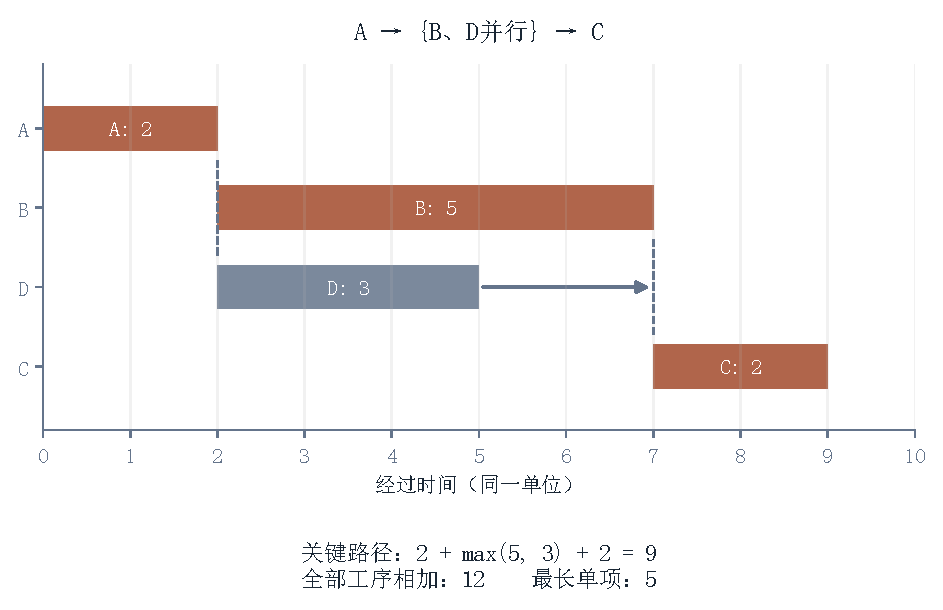
\includegraphics[width=\textwidth]{figures/critical-path.pdf}
\caption{A先执行，B与D随后并行，两项都完成后C才能开始。总历时为$2+\max(5,3)+2=9$，既不等于所有工序相加的12，也不等于最长单项的5。关键路径为A、B、C。}
\label{fig:mechanism-critical-path}
\end{figure}
\subsection{定位：大项与可改进项分别检查}

权重已知且刻度可比时，模型中较大的贡献项可以写为
\begin{equation}
c^\ast\in\operatorname*{arg\,max}_{c\in\{R,T,G\}}\alpha_c c,
\qquad(\alpha_R,\alpha_T,\alpha_G)=(\alpha,\beta,\gamma).
\label{eq:scale-dominant}
\end{equation}
未知权重时，不能仅凭哪个坐标的级数最大就宣布它主导总体黏滞。最大贡献项也未必是最值得优先改造的项，还要考察可行余量、成本、风险和相互作用。

在小幅、独立、边际成本近似固定的条件下，若压低一单位坐标$c$的成本为$\mu_c>0$，则
\begin{equation}
\frac{\alpha_c}{\mu_c}
\label{eq:scale-yield}
\end{equation}
比较的是每单位支出带来的模型内对数代价下降。它不是绝对净收益，也不处理跨维联动、有限预算、门槛与风险。有限项目仍须比较完整方案。

\begin{table}[ht]
\centering
\caption{从约束画像到改造选择}
\label{tab:scale-classes}
{\small
\begin{tabularx}{\textwidth}{@{}p{3.0cm}XX@{}}
\toprule
情形 & 要补的证据 & 可比较的行动\\
\midrule
主要约束可以低成本改善 & 改善幅度与全部成本 & 直接投入，并核验下游效果\\
改善会明显增加其他支出 & 联动幅度、承受者与风险 & 比较净效果及分配，重新设计接口\\
当前难改，但存在替代路径 & 替代任务、路线与结果标准 & 绕行、分阶段或缩小范围\\
多项约束同时偏高 & 全部可行路径与投入条件 & 重组方案，保留必要的等待与检验\\
\bottomrule
\end{tabularx}}
\end{table}

\subsection{示范一：低空服务的九个单元}

低空项目可以先拆成表\ref{tab:scale-lh}的九个单元。表中列的是应当查明的条件，具体等级要由选定机型、地区、运营范围与证据决定。

\begin{table}[ht]
\centering
\caption{低空服务：单元、约束与取证}
\label{tab:scale-lh}
{\small
\begin{tabularx}{\textwidth}{@{}p{3.2cm}XX@{}}
\toprule
单元 & 主要检查内容 & 应取得的证据\\
\midrule
电芯制造 & 配方、供给、良率与产能 & 产品规格、供应与生产记录\\
成组及热管理 & 系统质量、散热、故障隔离 & 包级测试与任务工况\\
机体及旋翼 & 材料、结构、制造与寿命 & 试验、工艺及维护依据\\
飞控与航电 & 功能、时延、失效与版本 & 需求、测试及审定记录\\
起降设施 & 场地、电力、接驳与备用 & 建设条件、接入与规划\\
运营维护 & 排班、备件、维修及恢复 & 运营设计与实测支持成本\\
适航审定 & 设计符合性与验证范围 & 对应辖区、型号与阶段文件\\
空域航路 & 运行边界、间隔与应急 & 适用规则及实际许可\\
服务接受 & 价格、噪声、可靠性与权益 & 对应人群的调查及运营反馈\\
\bottomrule
\end{tabularx}}
\end{table}

审定消耗人员、设备、试验与设施；协调和信任也需要物质载体与持续工作。不能因为输出是一份许可，就把资源记为零。公众接受需要定义人群和接受条件，不能先指定一个十年周期再据此预测落地。

把九个单元画成依赖图，区分可以并行的任务和必须等待的任务，再计算关键路径。电池改进可能同时改变载荷、备降裕量、经济性与审定证据；软件改进也可能减少试验负担。哪个环节控制投运时间，由项目的实际路径决定。

若许可仍在关键路径上，缩短不在该路径上的某道工序，可能不改变首次投运时间，却仍能降低费用或改善后续吞吐。把这几种结果分开，才能辨认改进究竟落在哪里。

\subsection{示范二：五类项目的比较入口}

\begin{table}[ht]
\centering
\caption{五类项目应分别核查的问题}
\label{tab:scale-five}
{\small
\begin{tabularx}{\textwidth}{@{}p{3.1cm}XX@{}}
\toprule
项目 & 资源与时间 & 依赖与确认\\
\midrule
大模型推理服务 & 现有容量、完整请求成本及扩容 & 输出触发什么下游行动\\
先进制程制造 & 设备、工序、良率与交付周期 & 哪些改动需要供应商与验证协同\\
低空服务 & 任务能耗、备份与设施条件 & 对应机型、空域和运营的证据\\
基因编辑治疗 & 递送、制造、观察与随访 & 细胞群体、临床终点与适用人群\\
水泥钢铁脱碳 & 工艺、能源、原料与更替周期 & 厂区、电力、运输、产品标准及需求\\
\bottomrule
\end{tabularx}}
\end{table}

同属一类项目，也可能采用不同技术路线和责任结构。基因编辑治疗不等于生殖系编辑，脱碳路线也不等于一种统一成熟工艺。先固定对象，再赋值与比较，行业名称只提供检索入口。

量表最终应当让争议落到具体证据上：哪个单元的什么条件改变了，依据是什么，哪些推论需要重算。能做到这一点，它就把总体判断变成了一份可复核的约束地图。
